\documentclass{article}

\usepackage{float}
\usepackage{graphicx}
\usepackage{hyperref}

\title{App to Download Data from Yahoo Finance's API}
\author{Bernardo Paulsen}

\begin{document}

\maketitle

\section{Introduction}

An app was implemented to downoad time series data from Yahoo Finance.

\section{App}

The app gets the ticker of the security in Yahoo Finance, the start date and end date. It returns the time series in a dataframe. It can also get multiple tickers and return a dataframe with information for all ticker.

\section{Test}

We test the app with brazilian stocks and with foreign stocks.

\subsection{Brazilian Stocks} 

Here we gather the data from six brazilian stocks: BBAS3, CESP6, JBSS3, IGTA3, EZTC3 and LAME4. We plot, for each stock, the adjusted close prices in Figure \ref{fig:br_adj} and the log returns in Figure \ref{fig:br_ret}.

\begin{figure}[H]
	\caption{Adjusted Close Prices}
	\label{fig:br_adj}
	\centering
	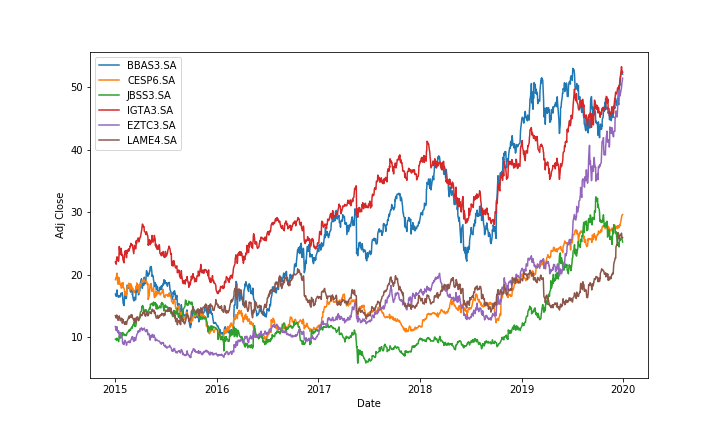
\includegraphics[width=\textwidth]{adj_close.png}
\end{figure}

\begin{figure}[H]
	\caption{Stocks' Returns}
	\label{fig:br_ret}
	\centering
	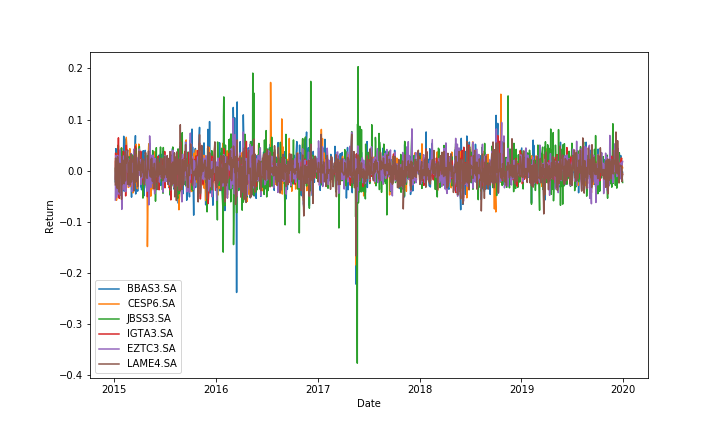
\includegraphics[width=\textwidth]{ret.png}
\end{figure}

\section{Foreign Stocks}

Here we gather the data from six foreign stocks: AAPL, ADBE, FB, KO, EBAY and EA. We plot, for each stock, the adjusted close prices in Figure \ref{fig:for_adj} and the log returns in Figure \ref{fig:for_ret}.

\begin{figure}[H]
	\caption{Adjusted Close Prices}
	\label{fig:for_adj}
	\centering
	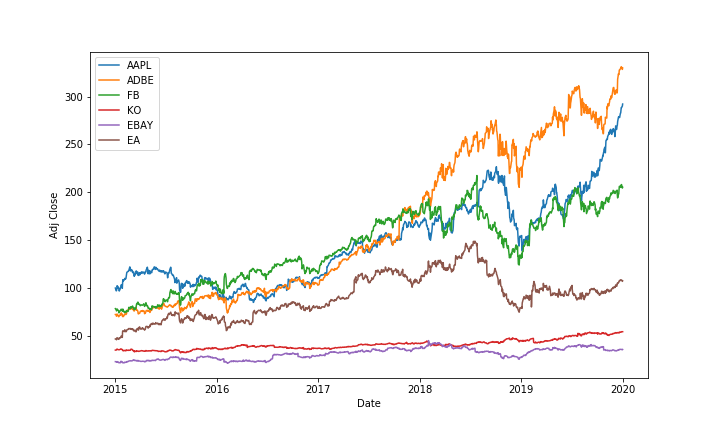
\includegraphics[width=\textwidth]{for_adj_close.png}
\end{figure}

\begin{figure}[H]
	\caption{Stocks' Returns}
	\label{fig:for_ret}
	\centering
	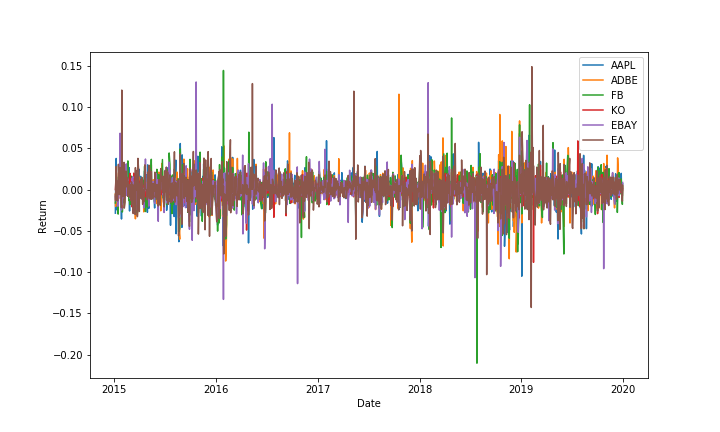
\includegraphics[width=\textwidth]{for_ret.png}
\end{figure}

\end{document}